\documentclass[11pt,fleqn]{book} % Default font size and left-justified equations
%%%%%%%%%%%%%%%%%%%%%%%%%%%%%%%%%%%%%%%%%
% The Legrand Orange Book
% Structural Definitions File
% Version 2.0 (9/2/15)
%
% Original author:
% Mathias Legrand (legrand.mathias@gmail.com) with modifications by:
% Vel (vel@latextemplates.com)
% 
% This file has been downloaded from:
% http://www.LaTeXTemplates.com
%
% License:
% CC BY-NC-SA 3.0 (http://creativecommons.org/licenses/by-nc-sa/3.0/)
%
%%%%%%%%%%%%%%%%%%%%%%%%%%%%%%%%%%%%%%%%%

%----------------------------------------------------------------------------------------
%	VARIOUS REQUIRED PACKAGES AND CONFIGURATIONS
%----------------------------------------------------------------------------------------

\usepackage[top=3cm,bottom=3cm,left=3cm,right=3cm,headsep=10pt,a4paper]{geometry} % Page margins

\usepackage{graphicx} % Required for including pictures
\graphicspath{{Pictures/}} % Specifies the directory where pictures are stored

\usepackage{lipsum} % Inserts dummy text

\usepackage{tikz} % Required for drawing custom shapes

\usepackage[spanish,activeacute,es-tabla]{babel}
%\usepackage[english]{babel} % English language/hyphenation

\usepackage{enumitem} % Customize lists
\setlist{nolistsep} % Reduce spacing between bullet points and numbered lists

\usepackage{booktabs} % Required for nicer horizontal rules in tables

\usepackage{xcolor} % Required for specifying colors by name
\definecolor{ocre}{RGB}{243,102,25} % Define the orange color used for highlighting throughout the book

%----------------------------------------------------------------------------------------
%	FONTS
%----------------------------------------------------------------------------------------

\usepackage{avant} % Use the Avantgarde font for headings
%\usepackage{times} % Use the Times font for headings
\usepackage{mathptmx} % Use the Adobe Times Roman as the default text font together with math symbols from the Sym­bol, Chancery and Com­puter Modern fonts

\usepackage{microtype} % Slightly tweak font spacing for aesthetics
\usepackage[utf8]{inputenc} % Required for including letters with accents
\usepackage[T1]{fontenc} % Use 8-bit encoding that has 256 glyphs

%----------------------------------------------------------------------------------------
%	BIBLIOGRAPHY AND INDEX
%----------------------------------------------------------------------------------------

\usepackage[style=alphabetic,citestyle=numeric,sorting=nyt,sortcites=true,
            autopunct=true,babel=hyphen,hyperref=true,abbreviate=false,
            backref=true,backend=biber]{biblatex}
\addbibresource{bibliography} % BibTeX bibliography file
\defbibheading{bibempty}{}

\usepackage{calc} % For simpler calculation - used for spacing the index letter headings correctly
\usepackage{makeidx} % Required to make an index
\makeindex % Tells LaTeX to create the files required for indexing

%----------------------------------------------------------------------------------------
%	MAIN TABLE OF CONTENTS
%----------------------------------------------------------------------------------------

\usepackage{titletoc} % Required for manipulating the table of contents

\contentsmargin{0cm} % Removes the default margin

% Part text styling
\titlecontents{part}[0cm]
{\addvspace{20pt}\centering\large\bfseries}
{}
{}
{}

% Chapter text styling
\titlecontents{chapter}[1.25cm] % Indentation
{\addvspace{12pt}\large\sffamily\bfseries} % Spacing and font options for chapters
{\color{ocre!60}\contentslabel[\Large\thecontentslabel]{1.25cm}\color{ocre}} % Chapter number
{\color{ocre}}  
{\color{ocre!60}\normalsize\;\titlerule*[.5pc]{.}\;\thecontentspage} % Page number

% Section text styling
\titlecontents{section}[1.25cm] % Indentation
{\addvspace{3pt}\sffamily\bfseries} % Spacing and font options for sections
{\contentslabel[\thecontentslabel]{1.25cm}} % Section number
{}
{\hfill\color{black}\thecontentspage} % Page number
[]

% Subsection text styling
\titlecontents{subsection}[1.25cm] % Indentation
{\addvspace{1pt}\sffamily\small} % Spacing and font options for subsections
{\contentslabel[\thecontentslabel]{1.25cm}} % Subsection number
{}
{\ \titlerule*[.5pc]{.}\;\thecontentspage} % Page number
[]

% List of figures
\titlecontents{figure}[0em]
{\addvspace{-5pt}\sffamily}
{\thecontentslabel\hspace*{1em}}
{}
{\ \titlerule*[.5pc]{.}\;\thecontentspage}
[]

% List of tables
\titlecontents{table}[0em]
{\addvspace{-5pt}\sffamily}
{\thecontentslabel\hspace*{1em}}
{}
{\ \titlerule*[.5pc]{.}\;\thecontentspage}
[]

%----------------------------------------------------------------------------------------
%	MINI TABLE OF CONTENTS IN PART HEADS
%----------------------------------------------------------------------------------------

% Chapter text styling
\titlecontents{lchapter}[0em] % Indenting
{\addvspace{15pt}\large\sffamily\bfseries} % Spacing and font options for chapters
{\color{ocre}\contentslabel[\Large\thecontentslabel]{1.25cm}\color{ocre}} % Chapter number
{}  
{\color{ocre}\normalsize\sffamily\bfseries\;\titlerule*[.5pc]{.}\;\thecontentspage} % Page number

% Section text styling
\titlecontents{lsection}[0em] % Indenting
{\sffamily\small} % Spacing and font options for sections
{\contentslabel[\thecontentslabel]{1.25cm}} % Section number
{}
{}

% Subsection text styling
\titlecontents{lsubsection}[.5em] % Indentation
{\normalfont\footnotesize\sffamily} % Font settings
{}
{}
{}

%----------------------------------------------------------------------------------------
%	PAGE HEADERS
%----------------------------------------------------------------------------------------

\usepackage{fancyhdr} % Required for header and footer configuration

\pagestyle{fancy}
\renewcommand{\chaptermark}[1]{\markboth{\sffamily\normalsize\bfseries\chaptername\ \thechapter.\ #1}{}} % Chapter text font settings
\renewcommand{\sectionmark}[1]{\markright{\sffamily\normalsize\thesection\hspace{5pt}#1}{}} % Section text font settings
\fancyhf{} \fancyhead[LE,RO]{\sffamily\normalsize\thepage} % Font setting for the page number in the header
\fancyhead[LO]{\rightmark} % Print the nearest section name on the left side of odd pages
\fancyhead[RE]{\leftmark} % Print the current chapter name on the right side of even pages
\renewcommand{\headrulewidth}{0.5pt} % Width of the rule under the header
\addtolength{\headheight}{2.5pt} % Increase the spacing around the header slightly
\renewcommand{\footrulewidth}{0pt} % Removes the rule in the footer
\fancypagestyle{plain}{\fancyhead{}\renewcommand{\headrulewidth}{0pt}} % Style for when a plain pagestyle is specified

% Removes the header from odd empty pages at the end of chapters
\makeatletter
\renewcommand{\cleardoublepage}{
\clearpage\ifodd\c@page\else
\hbox{}
\vspace*{\fill}
\thispagestyle{empty}
\newpage
\fi}

%----------------------------------------------------------------------------------------
%	THEOREM STYLES
%----------------------------------------------------------------------------------------

\usepackage{amsmath,amsfonts,amssymb,amsthm} % For math equations, theorems, symbols, etc

\newcommand{\intoo}[2]{\mathopen{]}#1\,;#2\mathclose{[}}
\newcommand{\ud}{\mathop{\mathrm{{}d}}\mathopen{}}
\newcommand{\intff}[2]{\mathopen{[}#1\,;#2\mathclose{]}}
\newtheorem{notation}{Notation}[chapter]

% Boxed/framed environments
\newtheoremstyle{ocrenumbox}% % Theorem style name
{0pt}% Space above
{0pt}% Space below
{\normalfont}% % Body font
{}% Indent amount
{\small\bf\sffamily\color{ocre}}% % Theorem head font
{\;}% Punctuation after theorem head
{0.25em}% Space after theorem head
{\small\sffamily\color{ocre}\thmname{#1}\nobreakspace\thmnumber{\@ifnotempty{#1}{}\@upn{#2}}% Theorem text (e.g. Theorem 2.1)
\thmnote{\nobreakspace\the\thm@notefont\sffamily\bfseries\color{black}---\nobreakspace#3.}} % Optional theorem note
\renewcommand{\qedsymbol}{$\blacksquare$}% Optional qed square

\newtheoremstyle{blacknumex}% Theorem style name
{5pt}% Space above
{5pt}% Space below
{\normalfont}% Body font
{} % Indent amount
{\small\bf\sffamily}% Theorem head font
{\;}% Punctuation after theorem head
{0.25em}% Space after theorem head
{\small\sffamily{\tiny\ensuremath{\blacksquare}}\nobreakspace\thmname{#1}\nobreakspace\thmnumber{\@ifnotempty{#1}{}\@upn{#2}}% Theorem text (e.g. Theorem 2.1)
\thmnote{\nobreakspace\the\thm@notefont\sffamily\bfseries---\nobreakspace#3.}}% Optional theorem note

\newtheoremstyle{blacknumbox} % Theorem style name
{0pt}% Space above
{0pt}% Space below
{\normalfont}% Body font
{}% Indent amount
{\small\bf\sffamily}% Theorem head font
{\;}% Punctuation after theorem head
{0.25em}% Space after theorem head
{\small\sffamily\thmname{#1}\nobreakspace\thmnumber{\@ifnotempty{#1}{}\@upn{#2}}% Theorem text (e.g. Theorem 2.1)
\thmnote{\nobreakspace\the\thm@notefont\sffamily\bfseries---\nobreakspace#3.}}% Optional theorem note

% Non-boxed/non-framed environments
\newtheoremstyle{ocrenum}% % Theorem style name
{5pt}% Space above
{5pt}% Space below
{\normalfont}% % Body font
{}% Indent amount
{\small\bf\sffamily\color{ocre}}% % Theorem head font
{\;}% Punctuation after theorem head
{0.25em}% Space after theorem head
{\small\sffamily\color{ocre}\thmname{#1}\nobreakspace\thmnumber{\@ifnotempty{#1}{}\@upn{#2}}% Theorem text (e.g. Theorem 2.1)
\thmnote{\nobreakspace\the\thm@notefont\sffamily\bfseries\color{black}---\nobreakspace#3.}} % Optional theorem note
\renewcommand{\qedsymbol}{$\blacksquare$}% Optional qed square
\makeatother

% Defines the theorem text style for each type of theorem to one of the three styles above
\newcounter{dummy} 
\numberwithin{dummy}{section}
\theoremstyle{ocrenumbox}
\newtheorem{theoremeT}[dummy]{Theorem}
\newtheorem{problem}{Problema}[chapter]    %CAMBIADO
\newtheorem{exerciseT}{Ejercicio}[chapter] %CAMBIADO
\theoremstyle{blacknumex}
\newtheorem{exampleT}{Ejemplo}[chapter]   %CAMBIADO
\theoremstyle{blacknumbox}
\newtheorem{vocabulary}{Vocabulary}[chapter]
\newtheorem{definitionT}{Definición}[section] %CAMBIADO
\newtheorem{corollaryT}[dummy]{Corollary}
\theoremstyle{ocrenum}
\newtheorem{proposition}[dummy]{Proposition}

%----------------------------------------------------------------------------------------
%	DEFINITION OF COLORED BOXES
%----------------------------------------------------------------------------------------

\RequirePackage[framemethod=default]{mdframed} % Required for creating the theorem, definition, exercise and corollary boxes

% Theorem box
\newmdenv[skipabove=7pt,
skipbelow=7pt,
backgroundcolor=black!5,
linecolor=ocre,
innerleftmargin=5pt,
innerrightmargin=5pt,
innertopmargin=5pt,
leftmargin=0cm,
rightmargin=0cm,
innerbottommargin=5pt]{tBox}

% Exercise box	  
\newmdenv[skipabove=7pt,
skipbelow=7pt,
rightline=false,
leftline=true,
topline=false,
bottomline=false,
backgroundcolor=ocre!10,
linecolor=ocre,
innerleftmargin=5pt,
innerrightmargin=5pt,
innertopmargin=5pt,
innerbottommargin=5pt,
leftmargin=0cm,
rightmargin=0cm,
linewidth=4pt]{eBox}	

% Definition box
\newmdenv[skipabove=7pt,
skipbelow=7pt,
rightline=false,
leftline=true,
topline=false,
bottomline=false,
linecolor=ocre,
innerleftmargin=5pt,
innerrightmargin=5pt,
innertopmargin=0pt,
leftmargin=0cm,
rightmargin=0cm,
linewidth=4pt,
innerbottommargin=0pt]{dBox}	

% Corollary box
\newmdenv[skipabove=7pt,
skipbelow=7pt,
rightline=false,
leftline=true,
topline=false,
bottomline=false,
linecolor=gray,
backgroundcolor=black!5,
innerleftmargin=5pt,
innerrightmargin=5pt,
innertopmargin=5pt,
leftmargin=0cm,
rightmargin=0cm,
linewidth=4pt,
innerbottommargin=5pt]{cBox}

% Creates an environment for each type of theorem and assigns it a theorem text style from the "Theorem Styles" section above and a colored box from above
\newenvironment{theorem}{\begin{tBox}\begin{theoremeT}}{\end{theoremeT}\end{tBox}}
\newenvironment{exercise}{\begin{eBox}\begin{exerciseT}}{\hfill{\color{ocre}\tiny\ensuremath{\blacksquare}}\end{exerciseT}\end{eBox}}				  
\newenvironment{definition}{\begin{dBox}\begin{definitionT}}{\end{definitionT}\end{dBox}}	
\newenvironment{example}{\begin{exampleT}}{\hfill{\tiny\ensuremath{\blacksquare}}\end{exampleT}}		
\newenvironment{corollary}{\begin{cBox}\begin{corollaryT}}{\end{corollaryT}\end{cBox}}	

%----------------------------------------------------------------------------------------
%	REMARK ENVIRONMENT
%----------------------------------------------------------------------------------------

\newenvironment{remark}{\par\vspace{10pt}\small % Vertical white space above the remark and smaller font size
\begin{list}{}{
\leftmargin=35pt % Indentation on the left
\rightmargin=25pt}\item\ignorespaces % Indentation on the right
\makebox[-2.5pt]{\begin{tikzpicture}[overlay]
\node[draw=ocre!60,line width=1pt,circle,fill=ocre!25,font=\sffamily\bfseries,inner sep=2pt,outer sep=0pt] at (-15pt,0pt){\textcolor{ocre}{R}};\end{tikzpicture}} % Orange R in a circle
\advance\baselineskip -1pt}{\end{list}\vskip5pt} % Tighter line spacing and white space after remark

%----------------------------------------------------------------------------------------
%	SECTION NUMBERING IN THE MARGIN
%----------------------------------------------------------------------------------------

\makeatletter
\renewcommand{\@seccntformat}[1]{\llap{\textcolor{ocre}{\csname the#1\endcsname}\hspace{1em}}}                    
\renewcommand{\section}{\@startsection{section}{1}{\z@}
{-4ex \@plus -1ex \@minus -.4ex}
{1ex \@plus.2ex }
{\normalfont\large\sffamily\bfseries}}
\renewcommand{\subsection}{\@startsection {subsection}{2}{\z@}
{-3ex \@plus -0.1ex \@minus -.4ex}
{0.5ex \@plus.2ex }
{\normalfont\sffamily\bfseries}}
\renewcommand{\subsubsection}{\@startsection {subsubsection}{3}{\z@}
{-2ex \@plus -0.1ex \@minus -.2ex}
{.2ex \@plus.2ex }
{\normalfont\small\sffamily\bfseries}}                        
\renewcommand\paragraph{\@startsection{paragraph}{4}{\z@}
{-2ex \@plus-.2ex \@minus .2ex}
{.1ex}
{\normalfont\small\sffamily\bfseries}}

%----------------------------------------------------------------------------------------
%	PART HEADINGS
%----------------------------------------------------------------------------------------

% numbered part in the table of contents
\newcommand{\@mypartnumtocformat}[2]{%
\setlength\fboxsep{0pt}%
\noindent\colorbox{ocre!20}{\strut\parbox[c][.7cm]{\ecart}{\color{ocre!70}\Large\sffamily\bfseries\centering#1}}\hskip\esp\colorbox{ocre!40}{\strut\parbox[c][.7cm]{\linewidth-\ecart-\esp}{\Large\sffamily\centering#2}}}%
%%%%%%%%%%%%%%%%%%%%%%%%%%%%%%%%%%
% unnumbered part in the table of contents
\newcommand{\@myparttocformat}[1]{%
\setlength\fboxsep{0pt}%
\noindent\colorbox{ocre!40}{\strut\parbox[c][.7cm]{\linewidth}{\Large\sffamily\centering#1}}}%
%%%%%%%%%%%%%%%%%%%%%%%%%%%%%%%%%%
\newlength\esp
\setlength\esp{4pt}
\newlength\ecart
\setlength\ecart{1.2cm-\esp}
\newcommand{\thepartimage}{}%
\newcommand{\partimage}[1]{\renewcommand{\thepartimage}{#1}}%
\def\@part[#1]#2{%
\ifnum \c@secnumdepth >-2\relax%
\refstepcounter{part}%
\addcontentsline{toc}{part}{\texorpdfstring{\protect\@mypartnumtocformat{\thepart}{#1}}{\partname~\thepart\ ---\ #1}}
\else%
\addcontentsline{toc}{part}{\texorpdfstring{\protect\@myparttocformat{#1}}{#1}}%
\fi%
\startcontents%
\markboth{}{}%
{\thispagestyle{empty}%
\begin{tikzpicture}[remember picture,overlay]%
\node at (current page.north west){\begin{tikzpicture}[remember picture,overlay]%	
\fill[ocre!20](0cm,0cm) rectangle (\paperwidth,-\paperheight);
\node[anchor=north] at (4cm,-3.25cm){\color{ocre!40}\fontsize{220}{100}\sffamily\bfseries\thepart}; 
\node[anchor=south east] at (\paperwidth-1cm,-\paperheight+1cm){\parbox[t][][t]{8.5cm}{
\printcontents{l}{0}{\setcounter{tocdepth}{0}} 
% CAMBIADO para que en la portada de cada capitulo solo salga la sección
}};
\node[anchor=north east] at (\paperwidth-1.5cm,-3.25cm){\parbox[t][][t]{15cm}{\strut\raggedleft\color{white}\fontsize{30}{30}\sffamily\bfseries#2}};
\end{tikzpicture}};
\end{tikzpicture}}%
\@endpart}
\def\@spart#1{%
\startcontents%
\phantomsection
{\thispagestyle{empty}%
\begin{tikzpicture}[remember picture,overlay]%
\node at (current page.north west){\begin{tikzpicture}[remember picture,overlay]%	
\fill[ocre!20](0cm,0cm) rectangle (\paperwidth,-\paperheight);
\node[anchor=north east] at (\paperwidth-1.5cm,-3.25cm){\parbox[t][][t]{15cm}{\strut\raggedleft\color{white}\fontsize{30}{30}\sffamily\bfseries#1}};
\end{tikzpicture}};
\end{tikzpicture}}
\addcontentsline{toc}{part}{\texorpdfstring{%
\setlength\fboxsep{0pt}%
\noindent\protect\colorbox{ocre!40}{\strut\protect\parbox[c][.7cm]{\linewidth}{\Large\sffamily\protect\centering #1\quad\mbox{}}}}{#1}}%
\@endpart}
\def\@endpart{\vfil\newpage
\if@twoside
\if@openright
\null
\thispagestyle{empty}%
\newpage
\fi
\fi
\if@tempswa
\twocolumn
\fi}

%----------------------------------------------------------------------------------------
%	CHAPTER HEADINGS
%----------------------------------------------------------------------------------------

% A switch to conditionally include a picture, implemented by  Christian Hupfer
\newif\ifusechapterimage
\usechapterimagetrue
\newcommand{\thechapterimage}{}%
\newcommand{\chapterimage}[1]{\ifusechapterimage\renewcommand{\thechapterimage}{#1}\fi}%
\newcommand{\autodot}{.}
\def\@makechapterhead#1{%
{\parindent \z@ \raggedright \normalfont
\ifnum \c@secnumdepth >\m@ne
\if@mainmatter
\begin{tikzpicture}[remember picture,overlay]
\node at (current page.north west)
{\begin{tikzpicture}[remember picture,overlay]
\node[anchor=north west,inner sep=0pt] at (0,0) {\ifusechapterimage\includegraphics[width=\paperwidth]{\thechapterimage}\fi};
\draw[anchor=west] (\Gm@lmargin,-9cm) node [line width=2pt,rounded corners=15pt,draw=ocre,fill=white,fill opacity=0.5,inner sep=15pt]{\strut\makebox[22cm]{}};
\draw[anchor=west] (\Gm@lmargin+.3cm,-9cm) node {\huge\sffamily\bfseries\color{black}\thechapter\autodot~#1\strut};
\end{tikzpicture}};
\end{tikzpicture}
\else
\begin{tikzpicture}[remember picture,overlay]
\node at (current page.north west)
{\begin{tikzpicture}[remember picture,overlay]
\node[anchor=north west,inner sep=0pt] at (0,0) {\ifusechapterimage\includegraphics[width=\paperwidth]{\thechapterimage}\fi};
\draw[anchor=west] (\Gm@lmargin,-9cm) node [line width=2pt,rounded corners=15pt,draw=ocre,fill=white,fill opacity=0.5,inner sep=15pt]{\strut\makebox[22cm]{}};
\draw[anchor=west] (\Gm@lmargin+.3cm,-9cm) node {\huge\sffamily\bfseries\color{black}#1\strut};
\end{tikzpicture}};
\end{tikzpicture}
\fi\fi\par\vspace*{270\p@}}}

%-------------------------------------------

\def\@makeschapterhead#1{%
\begin{tikzpicture}[remember picture,overlay]
\node at (current page.north west)
{\begin{tikzpicture}[remember picture,overlay]
\node[anchor=north west,inner sep=0pt] at (0,0) {\ifusechapterimage\includegraphics[width=\paperwidth]{\thechapterimage}\fi};
\draw[anchor=west] (\Gm@lmargin,-9cm) node [line width=2pt,rounded corners=15pt,draw=ocre,fill=white,fill opacity=0.5,inner sep=15pt]{\strut\makebox[22cm]{}};
\draw[anchor=west] (\Gm@lmargin+.3cm,-9cm) node {\huge\sffamily\bfseries\color{black}#1\strut};
\end{tikzpicture}};
\end{tikzpicture}
\par\vspace*{270\p@}}
\makeatother

%----------------------------------------------------------------------------------------
%	HYPERLINKS IN THE DOCUMENTS
%----------------------------------------------------------------------------------------

\usepackage{hyperref}
\hypersetup{hidelinks,backref=true,pagebackref=true,hyperindex=true,colorlinks=false,breaklinks=true,urlcolor= ocre,bookmarks=true,bookmarksopen=false,pdftitle={Title},pdfauthor={Author}}
\usepackage{bookmark}
\bookmarksetup{
open,
numbered,
addtohook={%
\ifnum\bookmarkget{level}=0 % chapter
\bookmarksetup{bold}%
\fi
\ifnum\bookmarkget{level}=-1 % part
\bookmarksetup{color=ocre,bold}%
\fi
}
}

%----------------------------------------------------------------------------------------
%	LISTADOS
%----------------------------------------------------------------------------------------
\usepackage{color}
\definecolor{gray97}{gray}{.97}
\definecolor{gray75}{gray}{.75}
\definecolor{gray45}{gray}{.45}

\usepackage{listings}
\lstset{
language=C,
frame=Ltb,
framerule=0pt,
aboveskip=0.5cm,
framextopmargin=3pt,
framexbottommargin=3pt,
framexleftmargin=0.4cm,
framesep=0pt,
rulesep=.4pt,
backgroundcolor=\color{gray97},
rulesepcolor=\color{black},
tabsize=2,
numbers=left,
numbersep=15pt,
numberstyle=\tiny,
numberfirstline = false,
breaklines=true,
%
identifierstyle=\color{blue},
stringstyle=\color{orange},
basicstyle=\footnotesize\ttfamily,
keywordstyle=\bfseries\color{green!40!black},
commentstyle=\itshape\color{purple!40!black},
%
showstringspaces = false,
commentstyle=\color{gray45},
literate=%
         {á}{{\'a}}1
         {é}{{\'a}}1
         {í}{{\'i}}1
         {ó}{{\'o}}1
         {ú}{{\'u}}1
         {ñ}{{\~n}}1
}

%----------------------------------------------------------------------------------------
%	MIS COSAS
%----------------------------------------------------------------------------------------
%\setlength{\parskip}{\baselineskip} % espaciado entre parrafos
\usepackage{subfig}

\begin{document}

%----------------------------------------------------------------------------------
% TITLE PAGE
%----------------------------------------------------------------------------------
\begingroup
\thispagestyle{empty}
\begin{tikzpicture}[remember picture,overlay]
\node[inner sep=0pt] (background) at (current page.center) {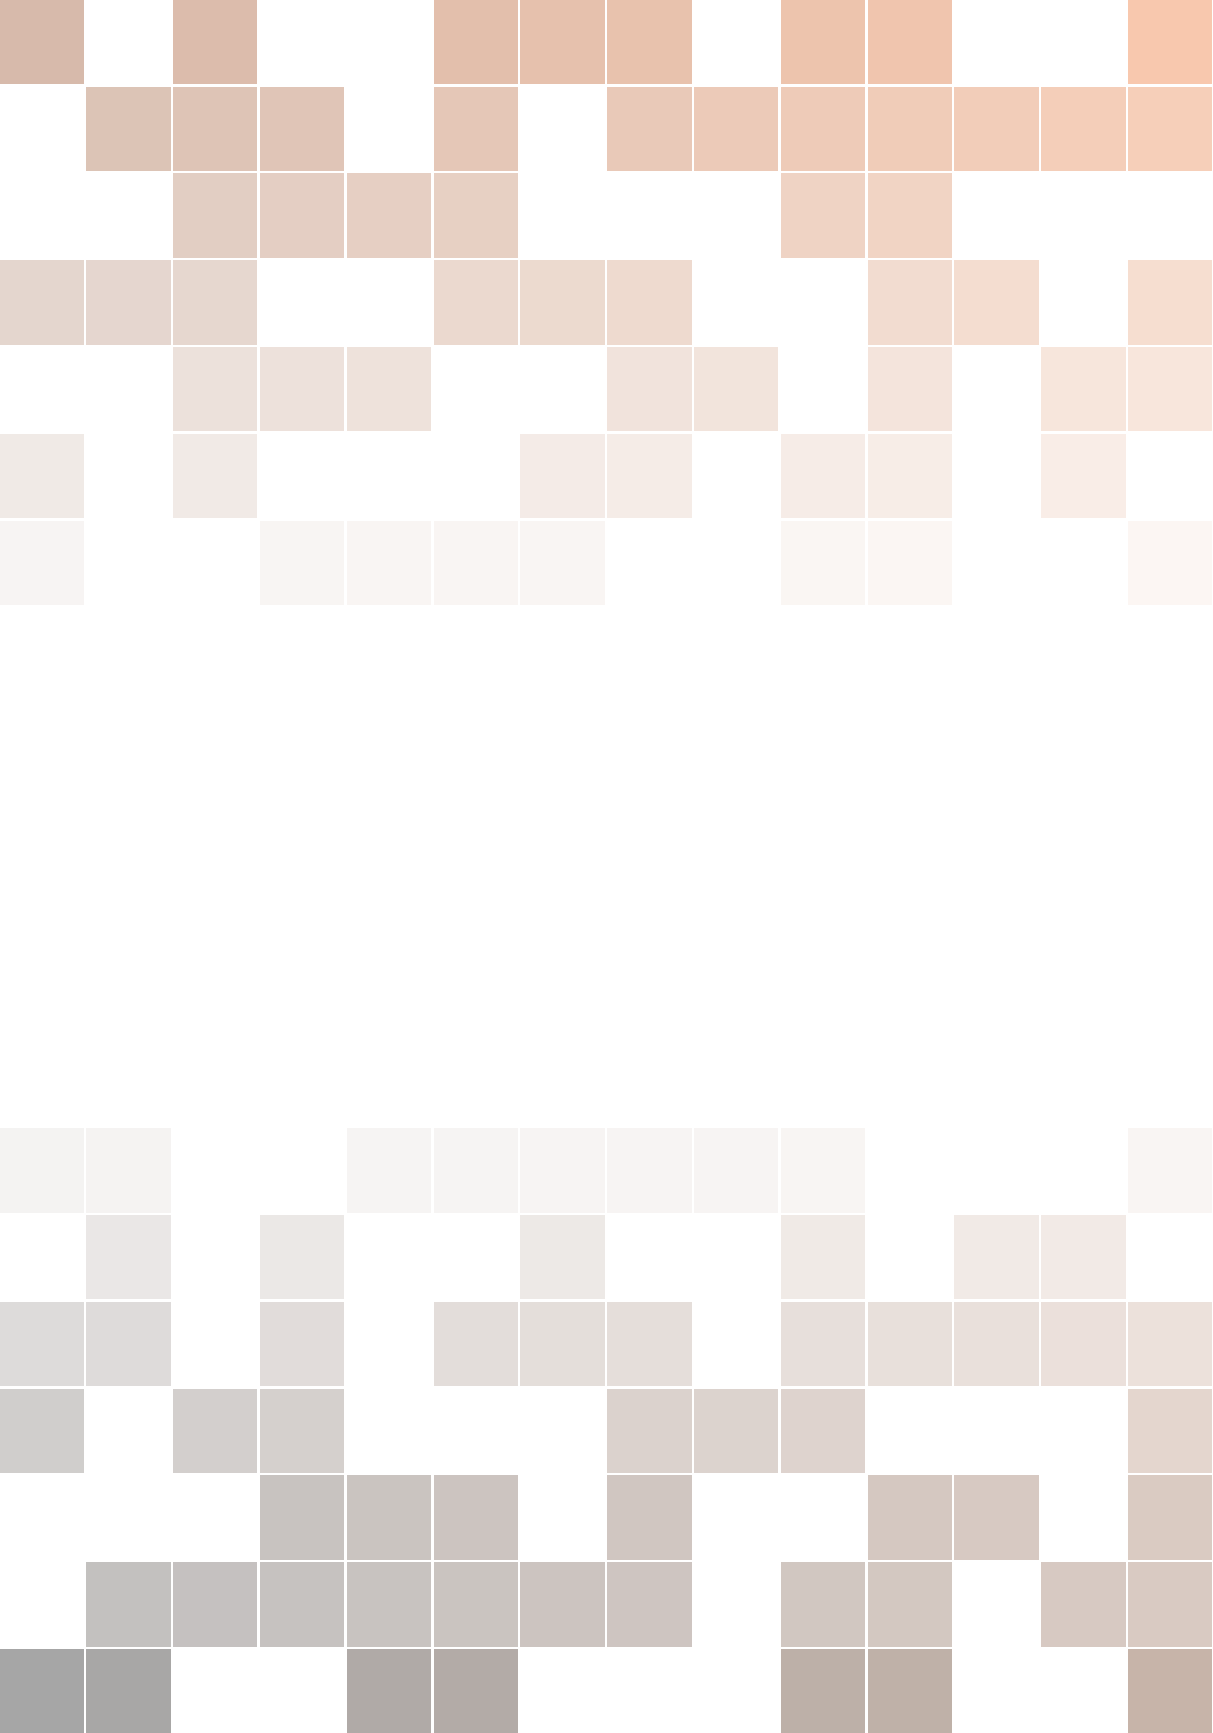
\includegraphics[width=\paperwidth]{background}};
\draw (current page.center) node [fill=ocre!30!white,fill opacity=0.6,text opacity=1,inner sep=1cm]
{\Huge\centering\bfseries\sffamily\parbox[c][][t]{\paperwidth}{\centering Programación de la Consola Nintendo DS\\[15pt] % Book title
{\Large VJ1214 Consolas y dispositivos de videojuegos}\\[20pt] % Subtitle
{\Large Grado en Diseño y Desarrollo de Videojuegos}\\[20pt] % Subtitle
{\huge Raúl Montoliu Colas\\ Juan Carlos Fernández Fernández\\ Maribel Castillo Catalán}}}; % Author name
\end{tikzpicture}
\vfill
\endgroup

%---------------------------------------------------------------------------------
% COPYRIGHT PAGE
%----------------------------------------------------------------------------------
\newpage
~\vfill
\thispagestyle{empty}

\noindent Copyright \copyright 2017 Raúl Montoliu Colas, Juan Carlos Fernández Fernández, Maribel Castillo Catalán. \\
\noindent Esta obra se distribuye bajo la Licencia \textit{Creative Commons Atribución-Compartir Igual 4.0 Internacional}. Puede consultat las condiciones de dicha licencia en: \url{http://creativecommons.org/licenses/by-sa/4.0/} \\

\includegraphics{Figuras/by-sa.png} 

%----------------------------------------------------------------------------------
% TABLE OF CONTENTS
%----------------------------------------------------------------------------------
\usechapterimagefalse % If you don't want to include a chapter image, use this to toggle images off - it can be enabled later with \usechapterimagetrue

\chapterimage{chapter_head_1.pdf} % Table of contents heading image
\pagestyle{empty} % No headers
\setcounter{tocdepth}{1} %Capitulos y secciones
\tableofcontents % Print the table of contents itself
\cleardoublepage % Forces the first chapter to start on an odd page so it's on the right
\pagestyle{fancy} % Print headers again

%----------------------------------------------------------------------------------
% CHAPTERS
%----------------------------------------------------------------------------------
\chapterimage{chapter_head_1.pdf} 
\chapter{Introducción a la consola Nintendo DS}

Este capítulo expone, en primer lugar, el conjunto de consolas de la familia Nintendo y posteriormente describe los principales elementos Hardware de la computadora Nintendo DS, que es la videoconsola a la que se hace referencia en el resto de los capítulos de este libro.

% -----------------------------------------------------------------
% -----------------------------------------------------------------
% -----------------------------------------------------------------
% -----------------------------------------------------------------
\section{Las videoconsolas de Nintendo}

Existe una amplia variedad de consolas de Nintendo:

\begin{itemize}
\item \textit{GameBoy Advance (GBA)}: tiene un procesador \textit{ARM7TDMI}, de 32 	bits, junto con un procesador \textit{Z80}, para dar soporte a los juegos de la \textit{GameBoy} clásica (ver Figura \ref{fig_c1_nintendo1}a). 
%
\item \textit{Nintendo DS (NDS)}: tiene un procesador ARM9 a 66Mhz y un procesador ARM7 a 33Mhz (ver Figura \ref{fig_c1_nintendo1}b).
%	
\item \textit{Nintendo DS Lite}: se diferencia de la NDS normal en su aspecto más estilizado, en mejoras de consumo energético y los diferentes niveles de control de brillo de la pantalla (ver Figura \ref{fig_c1_nintendo2}a). 
%	
\item \textit{Nintendo DSi}: incorpora dos cámaras de baja resolución, pantallas ligeramente mayores, mejor sonido, más memoria y una nueva ranura para tarjetas \textit{Secure Digital (SD)}. A cambio pierde la ranura de compa\-ti\-bilidad con los cartuchos de \textit{GameBoy	Advance (Slot2)} (ver Figura \ref{fig_c1_nintendo2}b).
%
\item \textit{Nintendo DSi XL}: conocida también como \textit{DSi XL}, es prácticamente idéntica a la anterior, salvo que su forma es significativamente mayor. 
%
\item \textit{Nintendo 3DS}: permite jugar con juegos y ver películas en 3D. Además, la nueva pantalla ofrece imágenes estereoscópicas sin necesidad de gafas especiales para disfrutar del efecto 3D. Incorpora una pantalla táctil, red inalámbrica ()\textit{WiFi}), sensor de movimiento con giroscopio de tres ejes y acelerómetro de tres ejes (ver Figura \ref{fig_c1_nintendo3}a).
%
\item \textit{Nintendo 2DS}: conserva las mismas funciones y especificaciones que la \textit{Nintendo 3DS}, salvo que no reproduce los videojuegos con efecto 3D, sino en 2D. Además, mantiene el tamaño de las pantallas de la \textit{Nintendo 3DS} (ver Figura \ref{fig_c1_nintendo3}b).
%	
\item \textit{New Nintendo 3DS}: esta consola cuenta con botones de colores.  Las pantallas de la \textit{New Nintendo 3DS} son 1,2 veces más grandes que las de la \textit{Nintendo 3DS} original, mientras que el tamaño de las pantallas de la \textit{New Nintendo 3DS XL} son similares a las de su predecesora. (ver Figura \ref{fig_c1_nintendo3}c). Las ranuras de la tarjeta de juego, del lápiz y del botón de encendido se han trasladado a la base de la consola. Como nuevas características cabe destacar:
	\begin{itemize}
		\item El rastreo facial para que la cámara siga la línea de visión del jugador, de esta forma se amplía la gama de ángulos desde los que se puede ver el efecto 3D estereoscópico del sistema.
		\item La variación automática del brillo de las pantallas según la iluminación ambiental.
		\item La transferencia inalámbrica de archivos multimedia entre la consola y un ordenador.
		\item Una CPU más potente, un ARM11 Dual Core a 532MHz. 
	\end{itemize}	
\end{itemize}


\begin{figure}
	\centering
	\subfloat[\textit{GameBoy Advance}]{
		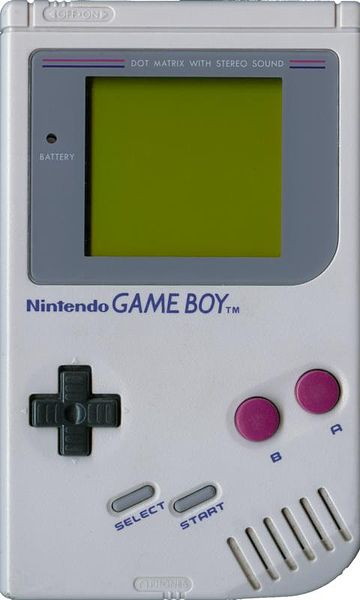
\includegraphics[height=5cm]{./Figuras/C1/c1_360px-Gameboy.jpg}}
	\subfloat[\textit{Nintendo DS}]{
		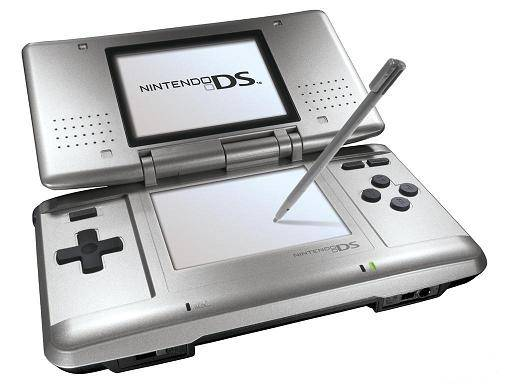
\includegraphics[height=5cm]{./Figuras/C1/c1_Nintendo_ds.jpg}}
	\caption{Videoconsolas de Nintendo: GBA y NDS}
	\label{fig_c1_nintendo1}
\end{figure}

\begin{figure}
	\centering
	\subfloat[\textit{Nintendo DS Lite}]{
		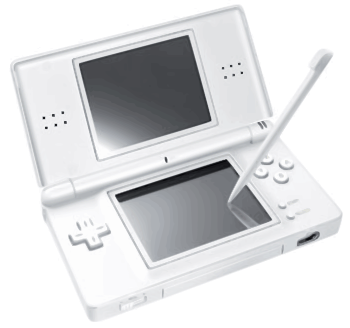
\includegraphics[height=5cm]{./Figuras/C1/c1_Nintendo-ds-lite.png}}
	\subfloat[\textit{Nintendo DSi}]{
		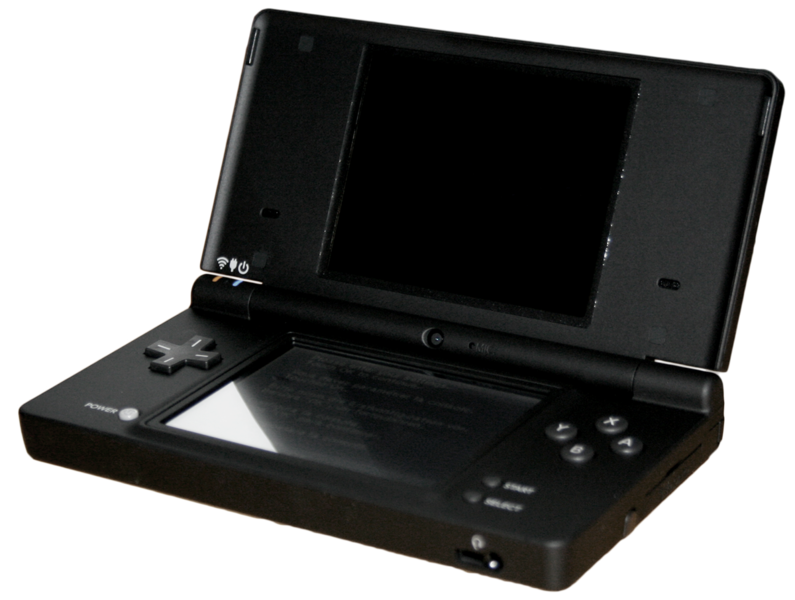
\includegraphics[height=5cm]{./Figuras/C1/c1_Nintendo_DSi.png}}
	\caption{Videoconsolas de Nintendo: NDSLite y NDSi}
	\label{fig_c1_nintendo2}
\end{figure}

\begin{figure}
	\centering
	\subfloat[\textit{Nintendo 3DS}]{
		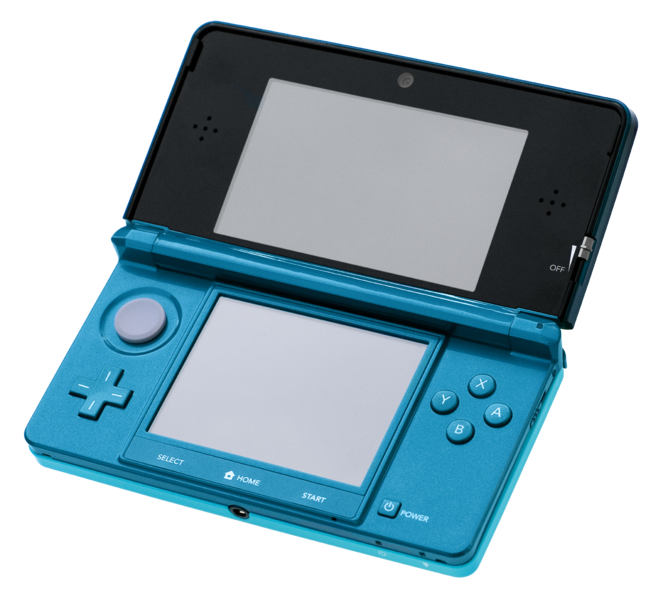
\includegraphics[height=4cm]{./Figuras/C1/c1_663px-Nintendo-3DS-AquaOpen.png}}
	\subfloat[\textit{Nintendo 2DS}]{
		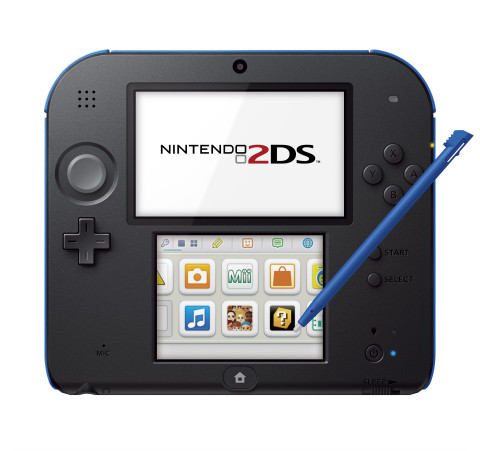
\includegraphics[height=4cm]{./Figuras/C1/c1_nintendo-2ds.jpg}}
	\subfloat[\textit{New Nintendo 3DS}]{
		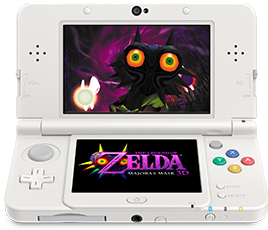
\includegraphics[height=4cm]{./Figuras/C1/c1_new-nintendo.png}}	
	\caption{Videoconsolas de Nintendo: N3DS, N2DS y NNew3DS}
	\label{fig_c1_nintendo3}
\end{figure}

% -----------------------------------------------------------------
% -----------------------------------------------------------------
% -----------------------------------------------------------------
% -----------------------------------------------------------------
\section{Hardware de la Nintendo DS (NDS)}

A continuación se describe el hardware de la \textit{Nintendo DS}:

\begin{itemize}
\item \textbf{Procesadores}: cuenta con dos procesadores, un ARM9 y un ARM7. El procesador ARM9 se encarga de la	lógica principal del programa, mientras que el ARM7, como procesador secundario, se encarga básicamente de gestionar el audio, la red inalámbrica (\textit{WiFi}) y algunas teclas. El hecho de que la consola NDS cuente con dos procesadores implica	la generación de dos ejecutables distintos, uno para cada procesador. El ejecutable del ARM7 actúa como esclavo del ARM9, atendiendo peticiones de reproducción de sonido o comunicaciones vía WiFi.
%	
\item \textbf{Memorias}:
	\begin{itemize}
	\item Memoria principal: tiene un tamaño de 4 MB. Dicha	memoria almacena el ejecutable para el ARM9, así como la gran mayoría de datos del ejecutable. Ambos procesadores pueden acceder a esta memoria en cualquier momento. Si ambos intentan acceder a la vez, será el que tenga mayor prioridad el que accede, quedando el otro a la espera.
	%
	\item Memoria de vídeo \textit{VRAM}: tiene  656 KB  distribuidos en  9 bancos de memoria de vídeo, que se pueden usar con diferentes propósitos. A lo largo de las sesiones de prácticas se verán más detalles de esta memoria de vídeo.
	%
	\item Otras memorias: tiene las pseudo-cachés \textit{WRAM} e \textit{IWRAM} de 96Kb, una memoria \textit{RAM} adicional para la \textit{BIOS} y una memoria virtual para vídeo (\textit{Virtual Video RAM}). 
	\end{itemize}
%
\item \textbf{Gráficos}: el hardware de vídeo se compone de dos núcleos gráficos 2D, uno	principal (\textit{main}) y otro secundario (\textit{sub}). Dichos núcleos se diferencian únicamente en que el motor principal puede \textit{renderizar} tanto la memoria de vídeo virtual sin utilizar el motor 2D, como mapas de bits de 256 colores, así como utilizar el motor 3D para el renderizado de alguno de sus fondos.
%
\item \textbf{Sonido}: dispone de altavoces estéreo y cuenta con 16 canales de audio independientes.
%
\item \textbf{Comunicación inalámbrica}: soporta el estándar de protocolo de comunicaciones \textit{IEEE 802.11}. El rango de comunicación inalámbrica varía de 10 a 30 metros, dependiendo de las circunstancias.
%
\item \textbf{Entrada/Salida}: tiene un puerto para cartuchos de juegos de Nintendo DS y otro para juegos de Game Boy Advance2. La NDS cuenta con una entrada para auriculares estéreo y otra entrada para micrófono.
%
\item \textbf{Doble pantalla}: las dos pantallas LCD son de 3 pulgadas. La pantalla inferior emplea tecnología táctil.
%
\item \textbf{Temporizador}: cuenta con un reloj de tiempo de real, que puede ser utilizado por una aplicación o juego para definir diferentes respuestas dependiendo de la hora del día.
\end{itemize}
 % 

%----------------------------------------------------------------------------------
% REFERENCES
%----------------------------------------------------------------------------------
\chapter*{Bibliography}
\addcontentsline{toc}{chapter}{\textcolor{ocre}{Bibliography}}
\section*{Books}
\addcontentsline{toc}{section}{Books}
\printbibliography[heading=bibempty,type=book]
\section*{Articles}
\addcontentsline{toc}{section}{Articles}
\printbibliography[heading=bibempty,type=article]
\end{document}
